% This file was created by matlab2tikz.
%
%The latest updates can be retrieved from
%  http://www.mathworks.com/matlabcentral/fileexchange/22022-matlab2tikz-matlab2tikz
%where you can also make suggestions and rate matlab2tikz.
%
\documentclass[tikz]{standalone}
\usepackage[T1]{fontenc}
\usepackage[utf8]{inputenc}
\usepackage{pgfplots}
\usepackage{grffile}
\pgfplotsset{compat=newest}
\usetikzlibrary{plotmarks}
\usepgfplotslibrary{patchplots}
\usepackage{amsmath}

\begin{document}
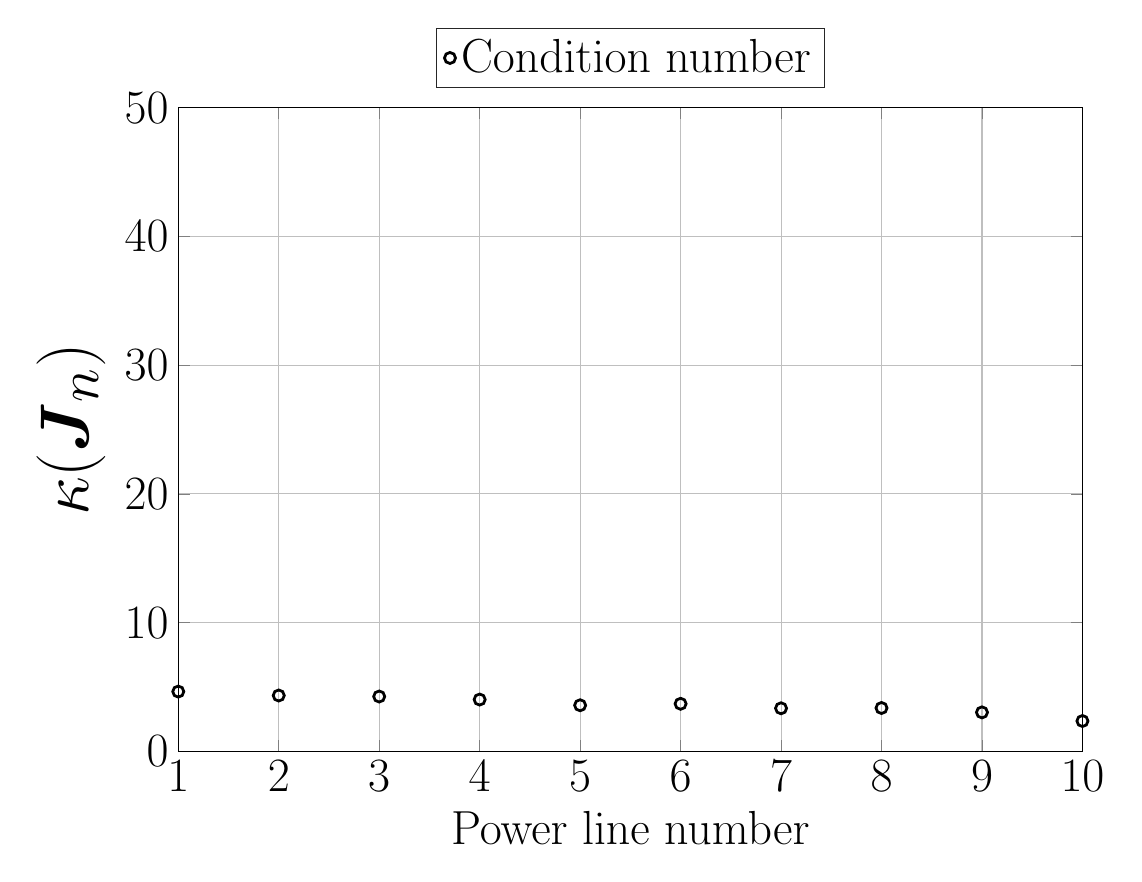
\begin{tikzpicture}

\begin{axis}[%
width=4.521in,
height=3.219in,
at={(0.758in,0.434in)},
scale only axis,
xmin=1,
xmax=10,
xlabel={Power line number},
xmajorgrids,
ymin=0,
ymax=50,
ylabel={$\kappa$(\mbox{\boldmath$J$}$_n$)},
ymajorgrids,
axis background/.style={fill=white},
legend style={at={(0.5,1.03)},anchor=south,legend cell align=left,align=left,draw=white!15!black},
xlabel style={font=\LARGE},ylabel style={font=\Huge},legend style={font=\LARGE},ticklabel style={font=\LARGE}
]
\addplot [color=black,line width=1.0pt,only marks,mark=o,mark options={solid}]
  table[row sep=crcr]{%
1	4.64523681642281\\
2	4.34031112589818\\
3	4.261847277491\\
4	4.02560140250221\\
5	3.58180441458692\\
6	3.69702267447058\\
7	3.34817777291077\\
8	3.36985419389401\\
9	3.02993190395761\\
10	2.35959548143542\\
};
\addlegendentry{Condition number};

\end{axis}
\end{tikzpicture}%
\end{document}